\section{Proposed Solution}

The solution proposed in this article centers around chunks of data which can be
organized by the user by means of different visualization models after being
inserted by the user from any data source supported by an implementation.

\subsection{Unstructured Chunks of Data}

Various types of unstructured data can be seen in figure \ref{fig:unstructdata}
but unstructured data doesn't oppose any restrictions upon the user or the
implementation of the user interaction concept itself. Basic implementations can
stick to text and graphical data. However, as the system grows so do the needs
of the user.

\begin{flfigure}
  \centering
    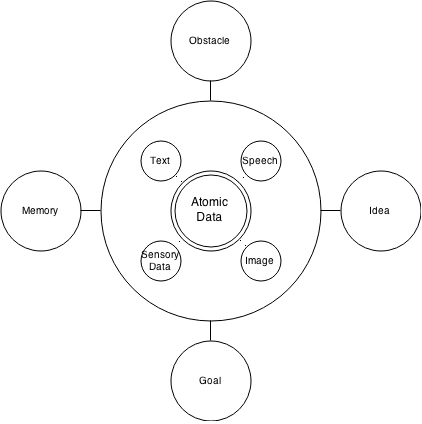
\includegraphics[width=0.9\linewidth]{00_resources/atomic_data.png}
    \caption{Unstructured data}
  \label{fig:unstructdata}
\end{flfigure}

Chunks of unstructured data can then be connected to other chunks by the user of
the system. The finer the chunks are, the more flexibility does the user have in
creating connections between chunks. A letter, for instance, can be inserted
into the system as one chunk of data which does not allow any connections within
the letter itself. However, the letter could also be inserted as multiple chunks
allowing the user to connect pieces of the letter to itself or other
information within the \gls{pims}.

\subsection{Data Sources}

In principle, any platform implementing a \gls{pims} that adheres to the
proposed concept can be a data source. However, this system is not meant to be
restricted to a particular platform but more so be a hub where any platform the
user chooses is supported in such a way that data can be inserted by the user.
Figure \ref{fig:datasources} shows a diagram of possible data sources across
multiple platforms.

\begin{flfigure}
  \centering
    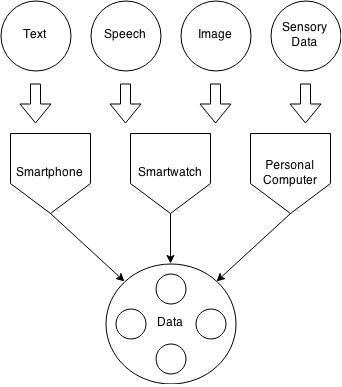
\includegraphics[width=0.9\linewidth]{00_resources/input_methods.png}
    \caption{Variety of data sources}
  \label{fig:datasources}
\end{flfigure}

\subsection{Organization of Data}

The organization of unstructured data is on a par with the available
visualizations within an implementation. That means that a \gls{pims}
implementing all presented visualizations allows the organization of unstructured
data by any of those visualizations or a combination thereof.

For instance, a system that supports connections between unstructured data and
a coordinate system must allow the user to connect chunks of unstructured data
with each other and simultaneously place these same chunks on a coordinate system.
A system need not support all visualizations presented in this paper or can
implement further visualizations not presented here.

\subsection{Connections of Data}

Chunks of unstructured data can be connected to other chunks as shown in figure
\ref{fig:visualconnections}. The visualization can resemble a two-dimensional
map showing all chunks of data including its connections or can lean toward a
radial graph where the user can move through the connections by changing the
chunk in the center.

\begin{flfigure}
  \centering
    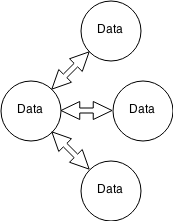
\includegraphics[width=0.5\linewidth]{00_resources/data_connections.png}
    \caption{Visualized relationships of unstructured data}
  \label{fig:visualconnections}
\end{flfigure}

\subsection{Labeling Data}

Figure \ref{fig:visuallabels} shows the organization of chunks of data by
folders, here called labels. The visual representation looks quite similar to
the figure but can take other forms.

\begin{flfigure}
  \centering
    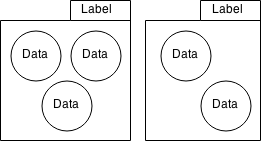
\includegraphics[width=0.5\linewidth]{00_resources/data_labels.png}
    \caption{Visualized labels of unstructured data}
  \label{fig:visuallabels}
\end{flfigure}

\subsection{Data Timeline}

Figure \ref{fig:visualtimeline} shows chunks of data within a timeline.
Organization using this model allows the user of the \gls{pims} to associate
chunks of data to relative or fixed points in time. Basically, this is a
one-dimensional coordinate system. Implementations do not have to restrict the
user to a timeline but can allow user-defined scales.

\begin{flfigure}
  \centering
    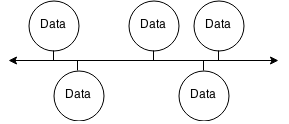
\includegraphics[width=0.5\linewidth]{00_resources/data_timeline.png}
    \caption{Visual timeline of unstructured data}
  \label{fig:visualtimeline}
\end{flfigure}

\subsection{Data within a Coordinate System}

Figure \ref{fig:visualcoordsys} shows a two-dimensional coordinate system with
chunks of data fixed to a certain point. This model must allow the user the
definition of the horizontal and vertical axis to allow a flexible use of the
coordinate system for multiple purposes. For instance, it can be used as the
\textit{importance-urgency matrix} or the \textit{growth-share matrix} but is
not restricted to those use cases.

\begin{flfigure}
  \centering
    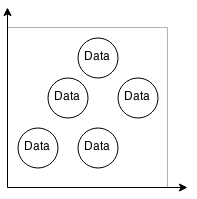
\includegraphics[width=0.5\linewidth]{00_resources/data_coord_system.png}
    \caption{Visual two-dimensional coordinate system of unstructured data}
  \label{fig:visualcoordsys}
\end{flfigure}

\subsection{Interaction with Visualization Models}

An implementation of the user interaction concept proposed here must allow the
user to interact with the visualizations. In particular, the user must be able
to organize chunks of data by interacting with the visualization itself. For
instance, connections must be changeable within the connections visualization or
chunks of data must be moveable within the coordinate system. How those
interactions are implemented is up to the implementation.

Furthermore, the user must be able to switch between visualizations easily.
There can be a collections of available visualization models for the user to
choose from but the user must also be able to switch to another visualization
by a pivotal chunk of unstructured data. For instance, a chunk of data which is
present in a connections visualization and a coordinate system can be used by
the user to switch to one of those visualizations. Whether the transition is
animated is up to the implementation. But if so, the pivotal chunk of data
should not disappear during the transition indicating to the user the pivotal
nature of this data chunk.
